
\documentclass{article}
\usepackage[margin=1.4in]{geometry}
\usepackage{color}
\usepackage{caption}
\usepackage{hyperref}
\usepackage{csquotes}
\usepackage{amsmath}
\usepackage{amssymb}
\usepackage{soul}
\usepackage{changepage}
\usepackage{alg}
\usepackage{graphicx}
\graphicspath{ {./} }
\usepackage{listings}
\lstset{aboveskip=3mm, belowskip=3mm, showstringspaces=false, columns=flexible, basicstyle={\small\ttfamily}, numbers=none, breaklines=true, breakatwhitespace=true, tabsize=3}

\usepackage{newlfont}
\usepackage{program}
\catcode`\_\active

\newcommand{\define}[1]{{\sc Definition.} \textbf{#1}: }

\begin{document}
\begin{center}{\huge   Fully General Computation in the Game of Life }\\[0.4cm]{\large  Philosophy of Computation Lab III }\\[0.75cm]{\large  Henry Blanchette }\\[0.5cm]{\large  March 22, 2019 }\\[1.0cm]\end{center} \tableofcontents\section{Turing Machine Structure}


The Turing Machine has been agreed upon as the manifestation of what is referred to when one talk of \textit{algorithm}. That is, a Turing Machine the simplest possible programming tool for formally transcribing algorithms. There are several equivalent ways to specify a Turing Machine, and I will describe; I will describe the canonical version. A canonical Turing Machine consists of a finite state machine (FSM), a tape, and a tape read head.





The finite state machine is specified by an alphabet (set of letters) $  \Sigma  $, a finite set of states $  Q  $, an initial state $  q_0 \in Q  $, a set of accept states $  F \subset Q  $, and a set of transitions $  \Delta \subseteq \{ f : \Sigma \times Q \rightarrow Q \times \{Left, Right\} \}  $. $  \Delta  $ describe how the FSM changes state given its current state and an input letter. The state machine encodes how the Turing Machine evolves over time and in what evolution step it is in at each point in time.





The tape is an infinite sequence of letters isomorphic to $  \mathbb{N}  $. That is, there is a beginning to the tape (entry 0), but no end. The Turing Machine begins operation with the input on the tape, starting from the beginning, and the rest of the tape after the input is filled with blank characters. The tape serves as a sort of infinite memory storage for the Turing Machine.





The Turing Machine accepts when the entire input has been read and the FSM is in an accept state. The Turing Machine rejects when the entire input has been read and the FSM is not in an accept state. The set of letter strings that a given Turing Machine accepts is the \textit{language} of the Turing Machine.





For example, consider the following Turing Machine with the alphabet $  \Sigma := \{ 0, 1 \}  $:



\begin{figure}[h]
\centering
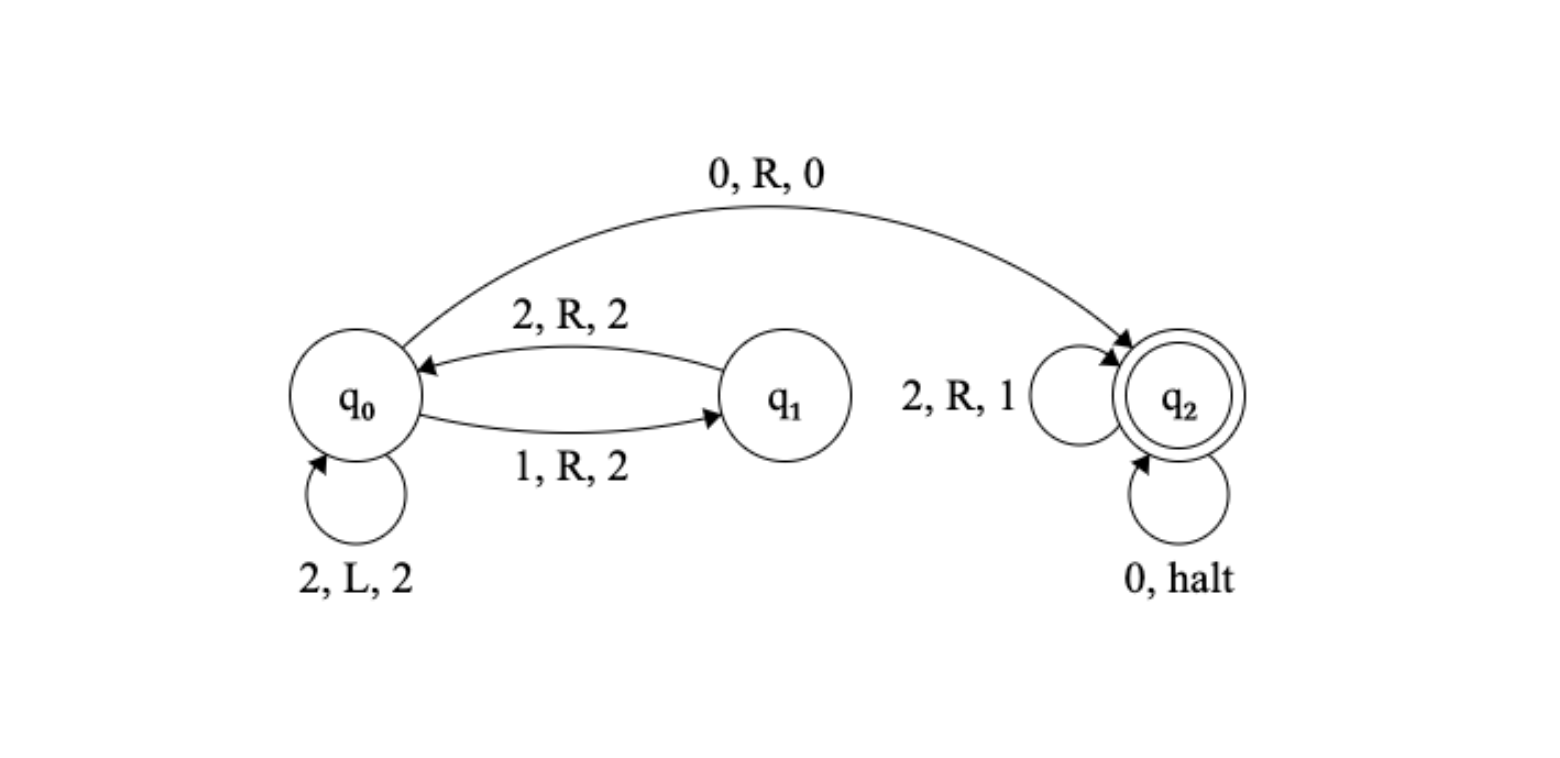
\includegraphics[width=10cm,keepaspectratio]{images/TM-example.png}
\captionsetup{labelformat=empty} \caption{A 3-stated 2-lettered Turing Machine.}
\end{figure}



It accepts a pattern of 1s (written as input on the tape), and leaves the tape with that pattern doubled. 


\section{A Turing Machine in the Game of Life}

This description is of all the modules required to build a generic Turing Machine in the Game of Life. However, the construction differs based on how many states are needed, how many letters are in the alphabet, and how much tape space is needed for the entire run of the machine. Notably, this last requirement is undecidable for Turing Machines in general.

\section{Computation in the Game of Life}\subsection{Spaceships}
\noindent\textbf{glider}: The smallest spaceship that travels diagonally by wagging its tail.

\vspace{1em}

\noindent\textbf{LWSS}: A lightweight spaceship that travels horizontally.

\vspace{1em}

\noindent\textbf{MWSS}: A middleweight spaceship that travels horizontally.

\vspace{1em}
\subsection{Spaceship Guns}
\noindent\textbf{P$X$}: Classifies a constant spaceship stream that contains a spaceship at $X$-generation intervals. For example, a P120 glider stream is a stream that contains a single glider at 120-generation intervals.

\vspace{1em}

\noindent\textbf{P$X$ $S$ GUN}: A spaceship gun that emits a P$X$ $S$ stream. For example, a P120 glider gun is a spaceship gun that emits a glider every 120-generations, maintaining a P120 glider stream.

\vspace{1em}

\begin{figure}[h]
\centering
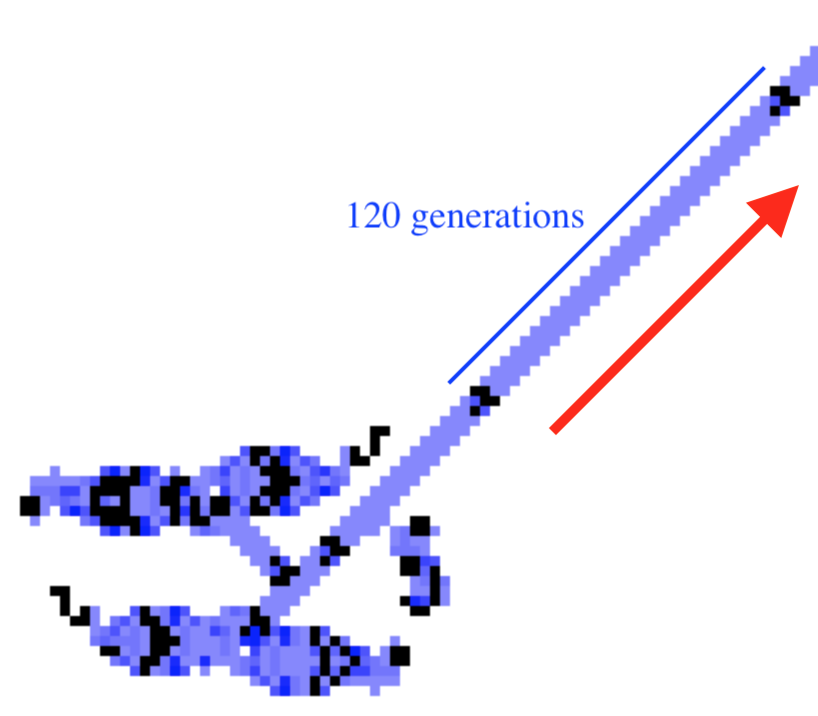
\includegraphics[width=10cm,keepaspectratio]{images/P120-GUN.png}
\captionsetup{labelformat=empty} \caption{A P120 glider gun}
\end{figure}
\subsection{Signals}
\noindent\textbf{Stream}: A constant, repeated output of spaceships in a line.

\vspace{1em}

\noindent\textbf{Signal}: A signal is some section of the stream that is present over some number of generations. \textbf{0} is encoded as an absent spaceship in signal. \textbf{1} is encoded by a present spaceship in the signal.

\vspace{1em}
\subsection{Signal Logic}
\noindent\textbf{Logic Gate}: A logic gate is defined by a logical function $  R  $ that takes as input 2 bits. When two input signals $  a, b  $ are sent into a logic gate, an output signal with the bits $  R(a_i, b_i)  $ where $  a_i, b_i  $ are the $  i\text{th}  $ bits of each input signal.

\vspace{1em}

\noindent\textbf{Reflector}: A reflector receives an input signal and then outputs a copy of that signal in some direction. The output signal may be modified in some way e.g. inverted or of a different spaceship type.

\vspace{1em}

\noindent\textbf{Signal Inversion}: An inverted signal is the \textbf{NOT} of a signal. Composing guns, reflectors, and gates often makes use of signal inversion. For example, many reflector implementations also invert their input signal, so referring to the inverted signal's state is useful.

\vspace{1em}

\noindent\textbf{Eater}: An eater receives as input a spaceship and then returns to the eater's original state. This process \textit{consumes} that spaceship without any trace leftover.

\vspace{1em}
\subsection{Design Outline for Rendell's Turing Machine}


The following sections will describe in detail how a specific style of Turing Machine can be constructed in the Game of Life. It is immensely complicated. Firstly, I will describe the basic outline of the Machine so that the details fit into a context that yields some purpose to their complexities. I will refer to this implementation of a Turing Machine in the Game of Life as RTM - Rendell's Turing Machine.





RTM is composed of the same parts described in the abstract description of a Turing Machine. RTM's TAPE is finite, however. The TAPE is split in half, where in the center is the TAPE read head apparatus. Each cell in the TAPE contains a value (alphabet letter), and the read head extracts that value at the beginning of every cycle (the POP part of the cycle) and sends it to the FSM.





The FSM consists of an $  n \times m  $ grid of MEMORY CELLs, where $  n  $ is the number of letters in the alphabet (including the blank letter) and $  m  $ is the number of states in the RTM. The MEMORY CELL at address $  (i,j)  $ corresponds to the transition from state $  i  $ given read letter $  j  $.





When the FSM receives the value read from the TAPE, it combines it with the stored current state. This data is converted into a MEMORY CELL address (i.e. ROW ADDRESS, COLUMN ADDRESS), and then taps the MEMORY CELL at that address. The MEMORY CELL has stored in it a signal that corresponds to the symbol to write and the direction to remove of the transition is represents.





The output of the tapped MEMORY CELL is sent back to the TAPE read head, where the PUSH part of the cycle writes the correct symbol onto the TAPE, and then moves the values along the tape one space according to the direction dictated by the transition. Altogether, this completes one cycle of the RTM.



\begin{figure}[h]
\centering
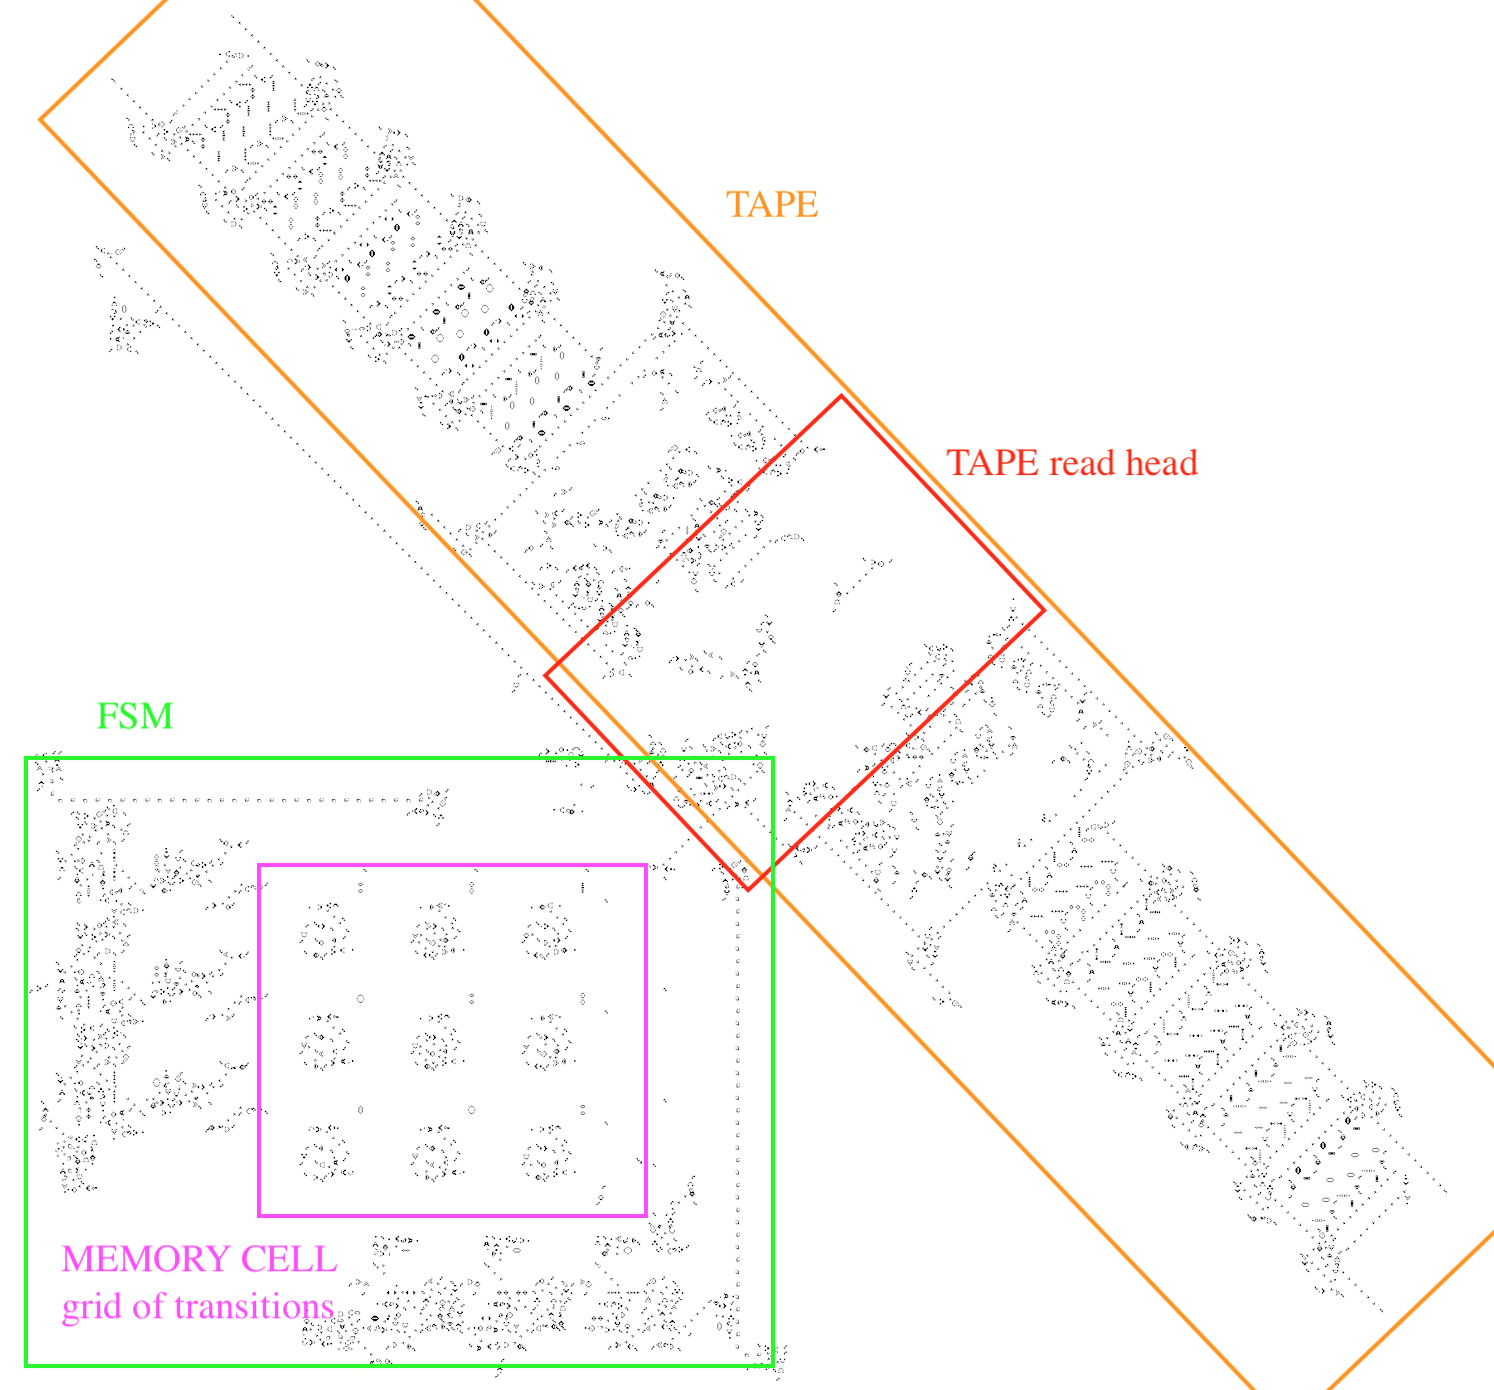
\includegraphics[width=10cm,keepaspectratio]{images/RTM.png}
\captionsetup{labelformat=empty} \caption{An example of an RTM. The Turing Machine that it encodes is the same as the example Turing Machine given in the Turing Machine Structure section.}
\end{figure}
\subsection{FINITE STATE MACHINE (FSM)}\subsubsection{Operation}

\begin{enumerate}
\item The SIGNAL DETECTOR sends the NEXT STATE message, part of which sends the ROW ADDRESS 1SSS.


\item The TAPE's OUTPUT COLLATOR sends the COLUMN ADDRESS 1VVV.


\item At the ROW ADDRESS, a MWSS is sent eastward. At the COLUMN ADDRESS, LWSS is sent northward. They collide, and their collision is formatted to trigger the memory cell selected by (ROW ADDRESSS, COLUMN ADDRESS).


\item The selected memory cell outputs a pattern of gliders to the northeastward.


\item A P30 MWSS GUN firing eastward is intercepted by the memory cell's output. The resulting MWSS stream heading eastward is the inverse of the memory cell's output.


\item The inverted memory cell output stream is intercepted by a northward MWSS stream, which inverts to yield the original memory cell output in the northward stream.


\item This final output stream is collected by the SIGNAL DETECTOR.

\end{enumerate}

\subsubsection{Components}
\noindent\textbf{ROW ADDRESS}: This signal has the form 1SSSS where SSSS is the address of the next state for the FSM. The signal is sent down the left side of the FSM. At the left-most side of each row of the FSM is a COMPARATOR that is configured to recognize its row's address. When the signal matches a row via a COMPARATOR, the signal is eaten and a MWSS is emitted to the right along the row, followed by an output collector that the MWSS triggers. The output collector interacts as a 1GAP8 blocking a P30 LWSS GUN. This allows 8 LWSS through that follow that original MWSS. This signal of 8 LWSS capture the output of the memory cell that the MWSS taps.

\vspace{1em}

\noindent\textbf{COLUMN ADDRESS}: This signal has the form 1VVV where VVV is the symbol just read from the TAPE. The inversion of this signal is sent by the OUTPUT COLLATOR to a P30 MWSS stream, un-inverting the signal and sending it across the bottom of the FSM. At the bottom of each column of the FSM is a COMPARATOR that is configured to recognize its column's address. When the signal matches a column via a COMPARATOR, the signal is eaten and a LWSS is emitted upward along the column (the output is converted to a LWSS via METAMORPHOSIS II).

\vspace{1em}

\noindent\textbf{MEMORY CELL}: Stores an 8-bit glider signal. The signal is continuously reflected around the interior walls of the cell, and a FANOUT copies the signal each output-frame. If the MEMORY CELL has not been tapped at the start of the output-frame, then the output signal is eaten. If the MEMORY CELL has not been tapped at the start of the output-frame, the output is not eaten and is successfully emitted.

\vspace{1em}

\noindent\textbf{COMPARATOR}: Receives an 8-bit signal and compares it to a stored signal value. The stores signal value is encoded in a MEMORY CELL. Each input-frame (8 time-steps), input and the the output from the MEMORY CELL is filtered through a NOT XOR gate and then sent into a SET RESET LATCH. A P240 GUN resets the latch every input-frame. The output is sampled by a glider from another P240 GUN right, slightly offset before the latch is reset, and this glider is destroyed if any bits of the input did not match the MEMORY CELL output. If all the bits did match, then the glider is successfully emitted. Note that the MEMORY CELL used here is slightly different from the MEMORY CELL used in the FSM - this MEMORY CELL repeatedly outputs its stored pattern whereas the FSM MEMORY CELL needs to be tapped before each output.

\vspace{1em}

\begin{figure}[h]
\centering
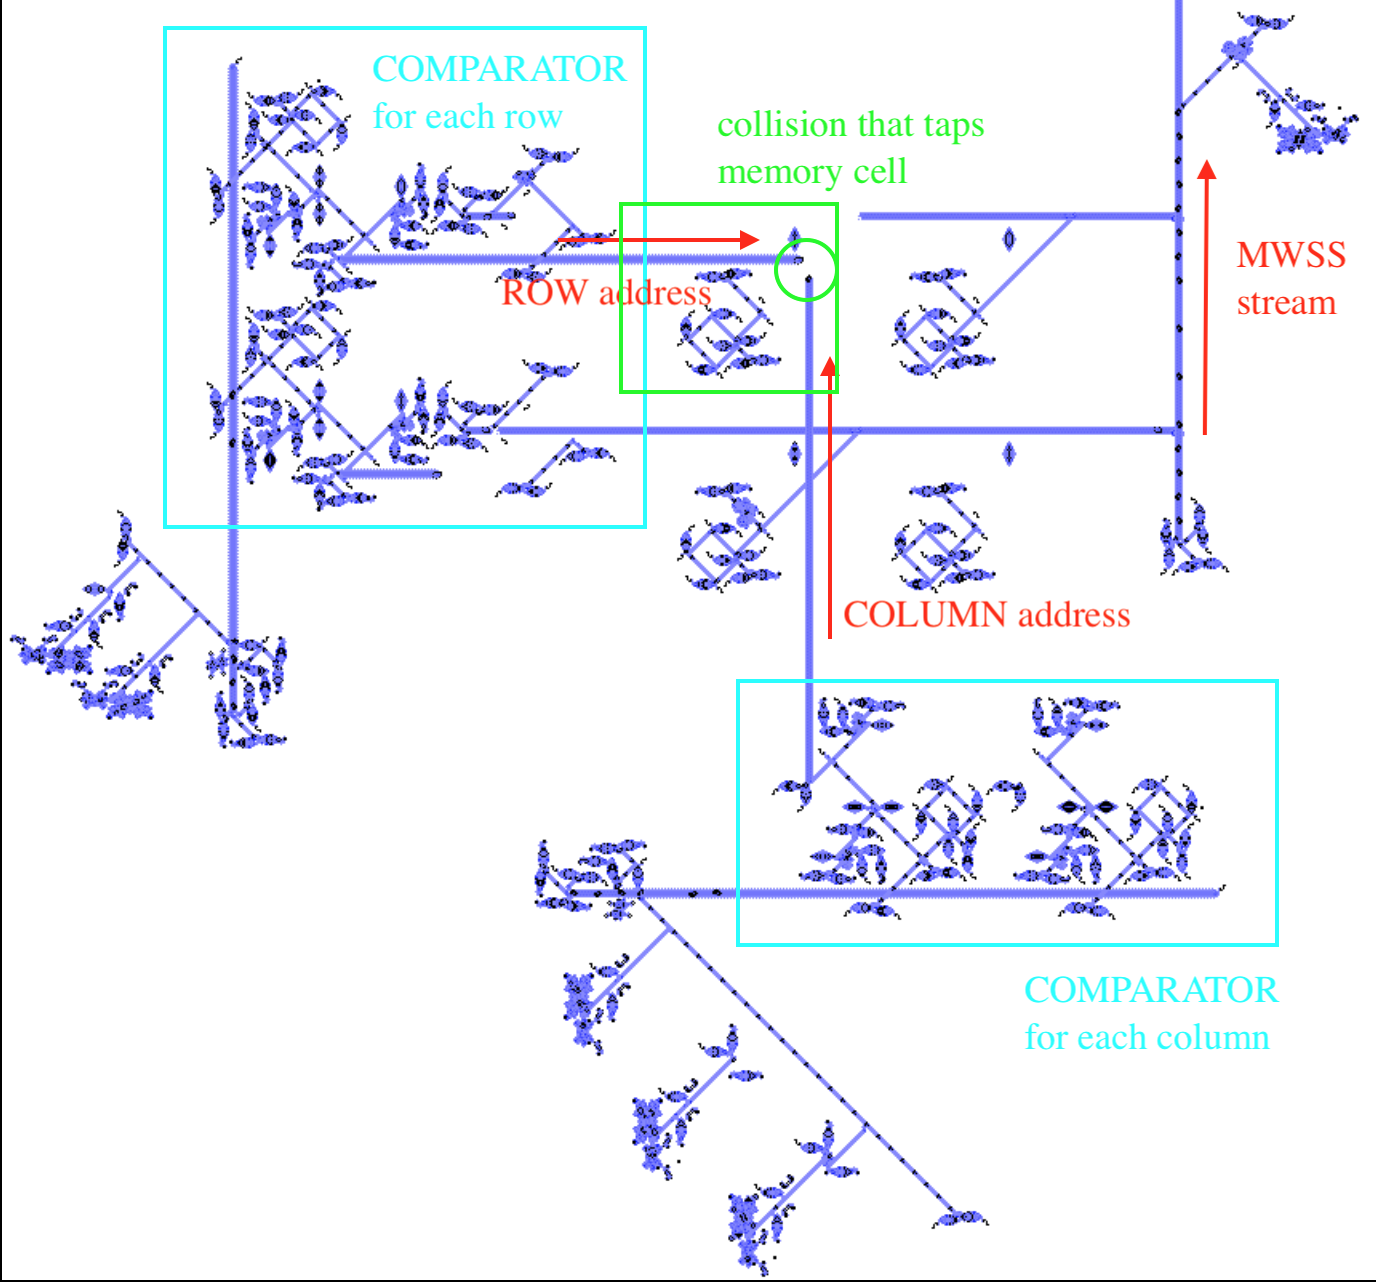
\includegraphics[width=10cm,keepaspectratio]{images/FSM.png}
\captionsetup{labelformat=empty} \caption{The FSM of the RTM.}
\end{figure}
\subsection{TAPE}


The TAPE is implemented as two stacks. In this way the finite state machine changes the position of the FSM's TAPE's read head by scrolling the TAPE's information left and right. The side of each stack closest to the TAPE's read head is called the CONTROL END.





There is no TAPE directly under the Read Head. A symbol extracted from the TAPE  into the FSM to be used as a state address during the Pop of one Cycle and then a symbol is inserted into the TAPE during the Push of the next Cycle.


\subsubsection{Operation}\begin{enumerate}
\item The output from the SIGNAL DETECTOR is copied once.


\item One output copy is sent to each STACK's CONTROL CONVERSION.


\item One of the STACK's OUTGATE is sent to the OUTPUT COLATOR.


\item The OUTPUT COLATOR sends this information to the FSM.

\end{enumerate}\subsubsection{Components}
\noindent\textbf{STACK}: Is composed of some number of STACK CELLs in sequence. There are two cycles for updating the TAPE: PUSH and POP. Control signals are passed up each side of the STACK. At each cell, a FANOUT copies the signal - one signal is inputted to the cell and the other is forwarded further along the STACK. The signal inputted into the cell is used to contain any VALUE that is contained in the cell, creating a sort of cell wall. The PUSH CONTROL and POP CONTROL interfere with this signal, nullifying 4 bits in this cell wall, allowing the VALUE GLIDER to be transfered from to an adjacent cell.
\begin{itemize}
\item  \textbf{PUSH}: All VALUE GLIDERs in the STACK are moved one cell away from the CONTROL END, freeing up a cell at the CONTROL END.
 

\item  \textbf{POP}: The VALUE GLIDER at the CONTROL END is removed and all VALUE GLIDERs in the STACK are moved one cell towards the CONTROL END, filling up the empty cell left by the removal.
 
\end{itemize}
\vspace{1em}

\noindent\textbf{VALUE GLIDER}: Each stack cell has an interior that is capable of holding a VALUE GLIDER. The cell's walls, streams of gliders, reflect the VALUE GLIDER back and forth so that it is contained inside the stack cell. When one of the cell's walls is disrupted (a gap created by the PUSH CONTROL or POP CONTROL), the VALUE GLIDER is allowed to move in one direction along the TAPE into another stack cell. The only case when the VALUE GLIDER would exit the TAPE (the TAPE is finite) is when it is being popped (as part of POP) or when it goes off the non-CONTROL END, in which case it is released into the ether to be forgotten (include a larger tape if you need more space).

\vspace{1em}

\noindent\textbf{OUTGATE}: A P120 GLIDER GUN tests for a 4-glider gap in the STACK's control stream, which is put there by POP CONTROL. On the occurrence of such a gap, the output of the gun gets through and triggers a 1GAP4 gate that samples for the 4 bits in an inverted copy of the cell wall. The gun additionally expands the gap by 1 bit, and includes this n the output of the OUTGATE. The output is of the form 1VVV - an address for the FSM.

\vspace{1em}

\noindent\textbf{OUTPUT COLATOR}: Inverts each STACK OUTGATE output and feeds it to the COLUMN ADDRESS of the FSM.

\vspace{1em}

\noindent\textbf{POP CONTROL}: Is a signal with a single glider (indicating that a POP should be initiated). It is sent along the TAPE and creates a gap in the control-side cell wall of each cell, allowing the contained VALUE GLIDERS to translate one cell towards the CONTROL END of the TAPE. At the CONTROL END of the tape, the bit in the CONTROL CELL is released and tested by the INGATE, which indicates if the CONTROL CELL's value was a 0 or 1.

\vspace{1em}

\noindent\textbf{PUSH CONTROL}: Is a signal with a single glider (indicating that a PUSH should be initiated). It is sent along the TAPE and creates a gap in the control-opposite-side cell wall of each cell, allowing the contained VALUE GLIDERS to translate one cell away from the CONTROL END of the TAPE. This leaves empty the CONTROL CELL.

\vspace{1em}

\noindent\textbf{CONTROL CELL}: The stack cell furthest to the control end (right next to the STACK read head section).

\vspace{1em}

\begin{figure}[h]
\centering
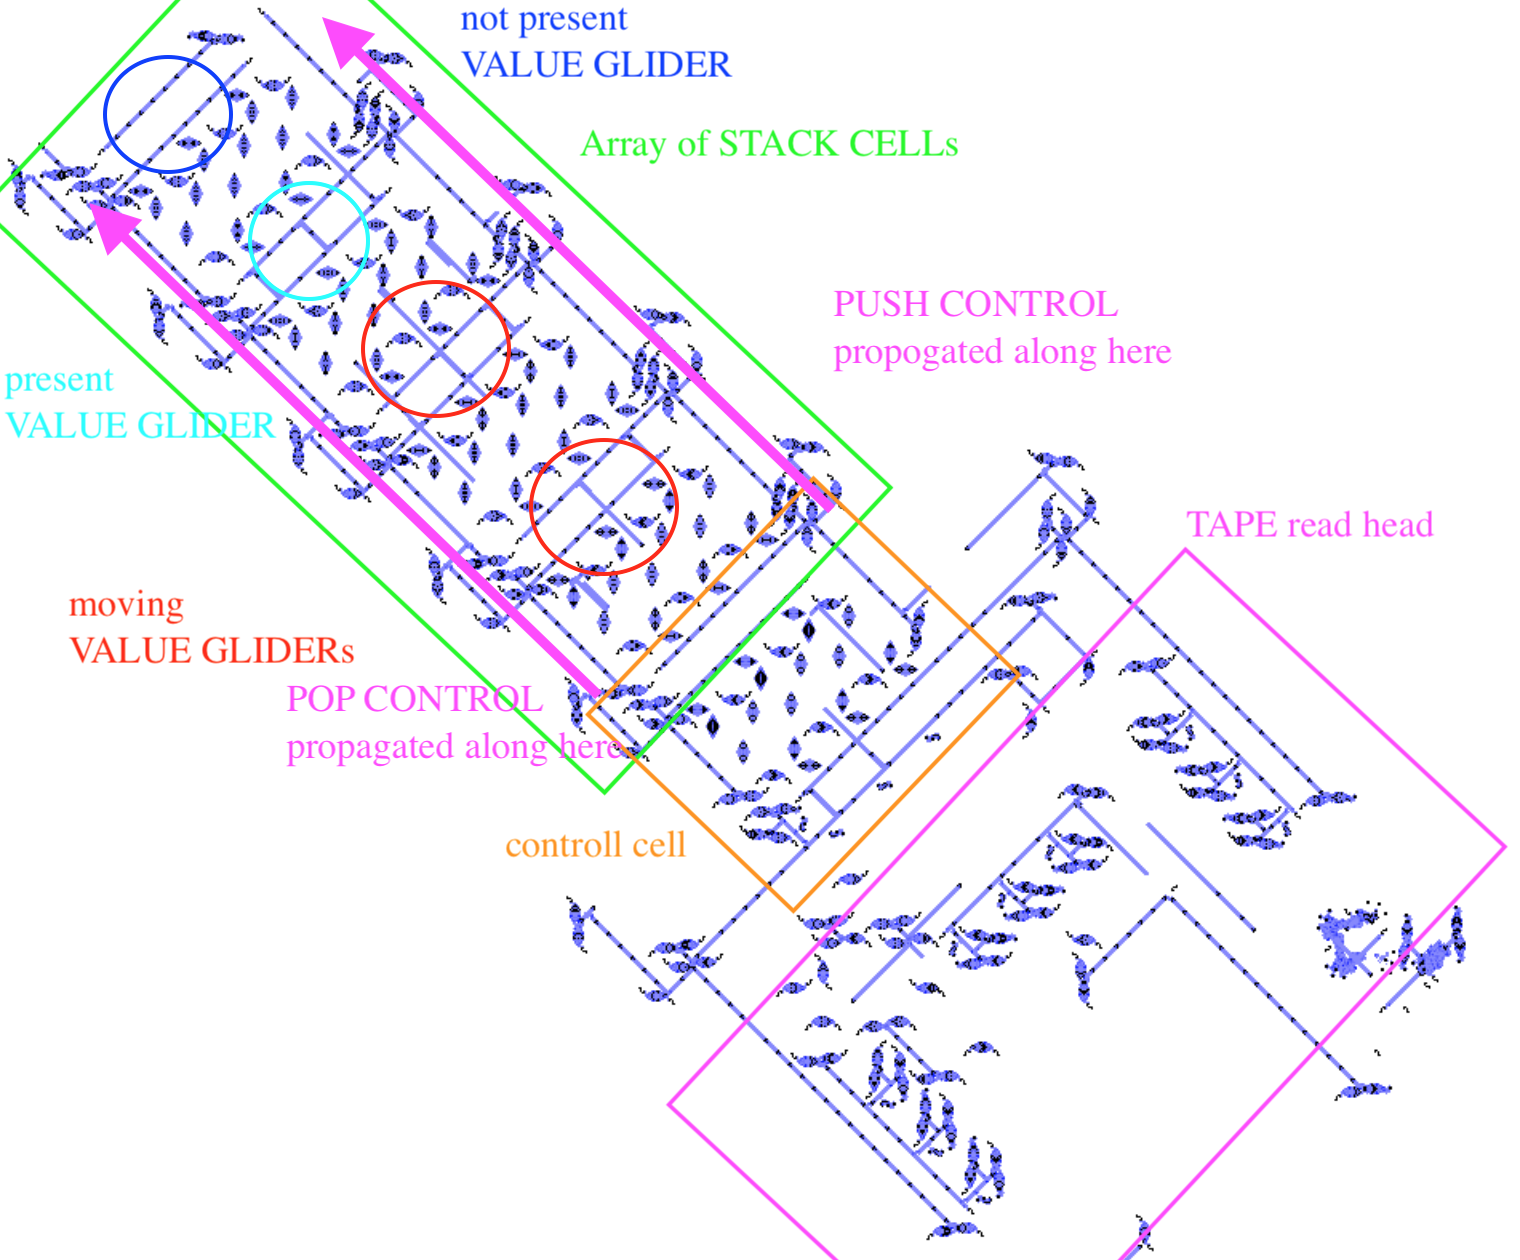
\includegraphics[width=10cm,keepaspectratio]{images/TAPE.png}
\captionsetup{labelformat=empty} \caption{The TAPE of the RTM.}
\end{figure}
\subsection{SIGNAL DETECTOR}


The SIGNAL DETECTOR joins the FSM to the TAPE.
\begin{itemize}
\item Detects output from the FSM and generates the input for the CONTROL CONVERSION.


\item Sends NEXT STATE from OUTPUT COLLATOR to FSM

\end{itemize}

\subsubsection{Operation}

\begin{enumerate}
\item Receives an input glider signal. The signal has two 1s on its ends, with some number of 0s between them. In gliders, this looks like two gliders that are some variable distance apart (the distance is divisible by the time-set of and within a certain specific to the SIGNAL DETECTOR).


\item Inverts the signal and uses a FANOUT to split it into two signals heading in opposite directions.


\item Each inverted copy of the signal interacts with some gates and reflectors to un-invert in the form of two output signals. The two output signals differ depending on the input signal.


\item One output is sent to the CONTROL CONVERSION


\item The other output is combined with a copy of the original input to convert the DVVVSSSS signal to DVV1SSSS so that 1SSS can be used to address the FSM. The D encodes the direction of the transition (left or right), the VVV encodes the letter value just read, and the SSSS encodes the next state. This output is sent to NEXT STATE DELAY.

\end{enumerate}

\subsubsection{Components}
\noindent\textbf{SET RESET LATCH}: Receives glider input signals from two sources: on and off. When a signal is received from the on-input and the LATCH is in state OFF, the LATCH begins emitting a stream of constant 1s. When a signal is received from the off-input and LATCH is in state ON, the LATCH stops emitting a stream of 1s (i.e. begins emitting a stream of 0s instead).

\vspace{1em}

\begin{figure}[h]
\centering
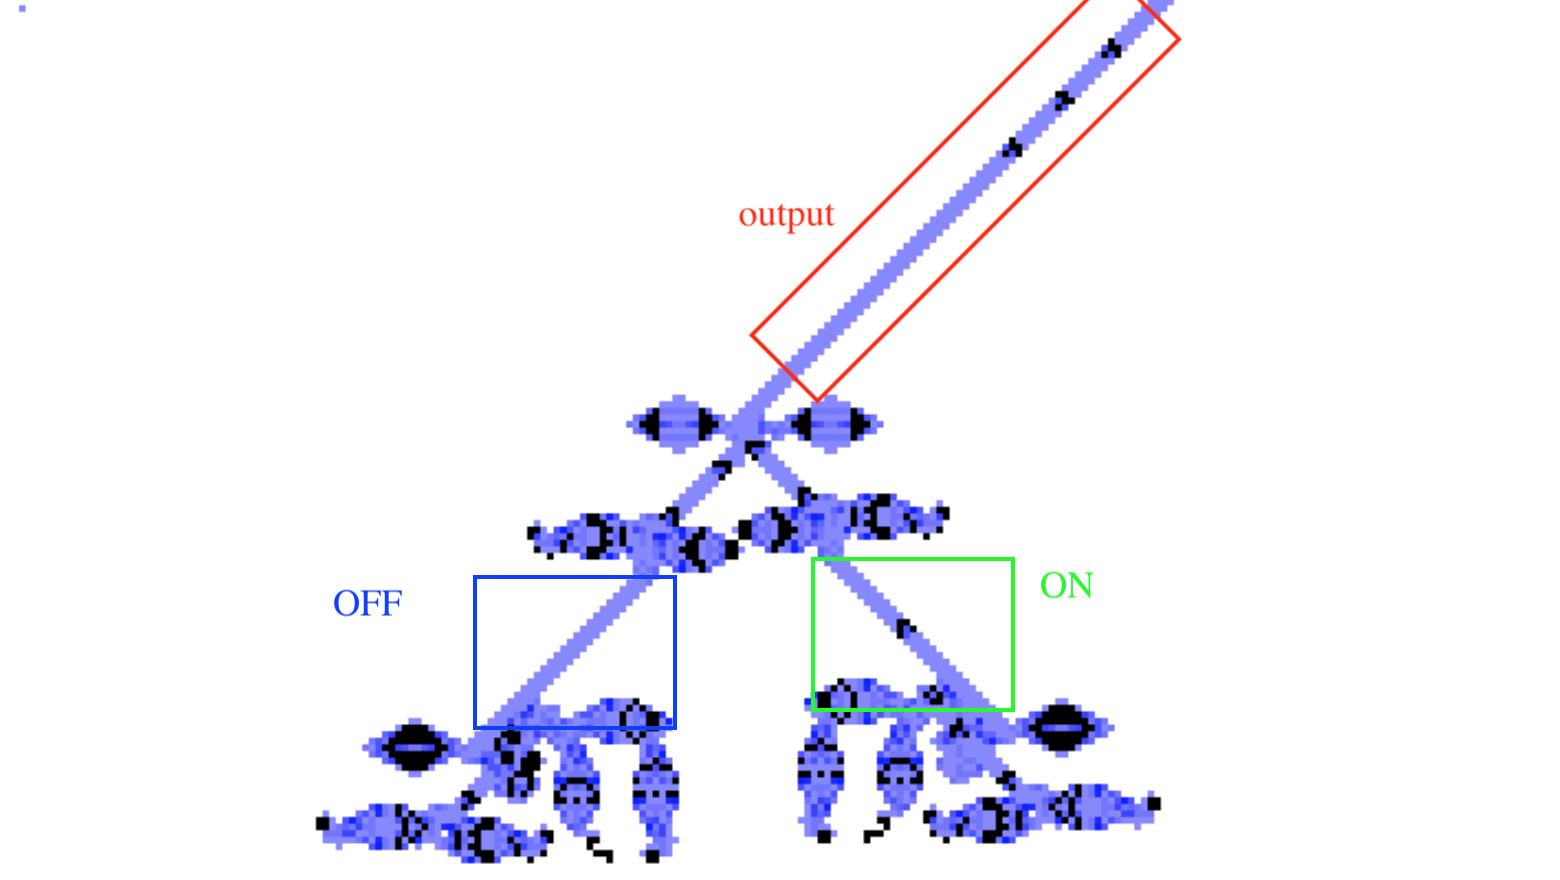
\includegraphics[width=10cm,keepaspectratio]{images/SET-RESET-LATCH.png}
\captionsetup{labelformat=empty} \caption{A SET RESET LATCH}
\end{figure}

\noindent\textbf{CONTROL CONVERSION}: Each STACK has a different implementation of this; one performs a PUSH and the other performs a POP. Receives two input from SIGNAL DETECTOR: One input is a glider stream with 9 gliders with the form DVVVSSSS where D is the direction for POP/PUSH, VVV is the symbol to POP/PUSH and SSSS is the NEXT STATE for the FSM. The other input is is a glider indicating that a signal has been received.



A P240 GLIDER GUN receives a NOT D glider from the inverted DVVVSSSS signal to produce an output but only when D is nonzero. This is passed on to a FANOUT, which outputs two copies of the signal - one two the PUSH/POP CONTROL of the STACK and the other (a single glider) towards the other input from the SIGNAL DETECTOR to delete it. This SIGNAL DETECTOR is either for the PUSH CONTROL or POP CONTROL of the STACK.



\vspace{1em}

\noindent\textbf{NEXT STATE DELAY}: A long loop that delays the NEXT STATE signal so that the address signal to is received by the FSM in parallel with the TAPE's output. The TAPE's output is originally DVV1SSSS, but along its way to the FSM, it is modified by a 1GAP3 powered by a P240 GLIDER GUN which removes the DVV from the signal, leaving 1SSSS for input into the ROW ADDRESS.

\vspace{1em}

\begin{figure}[h]
\centering
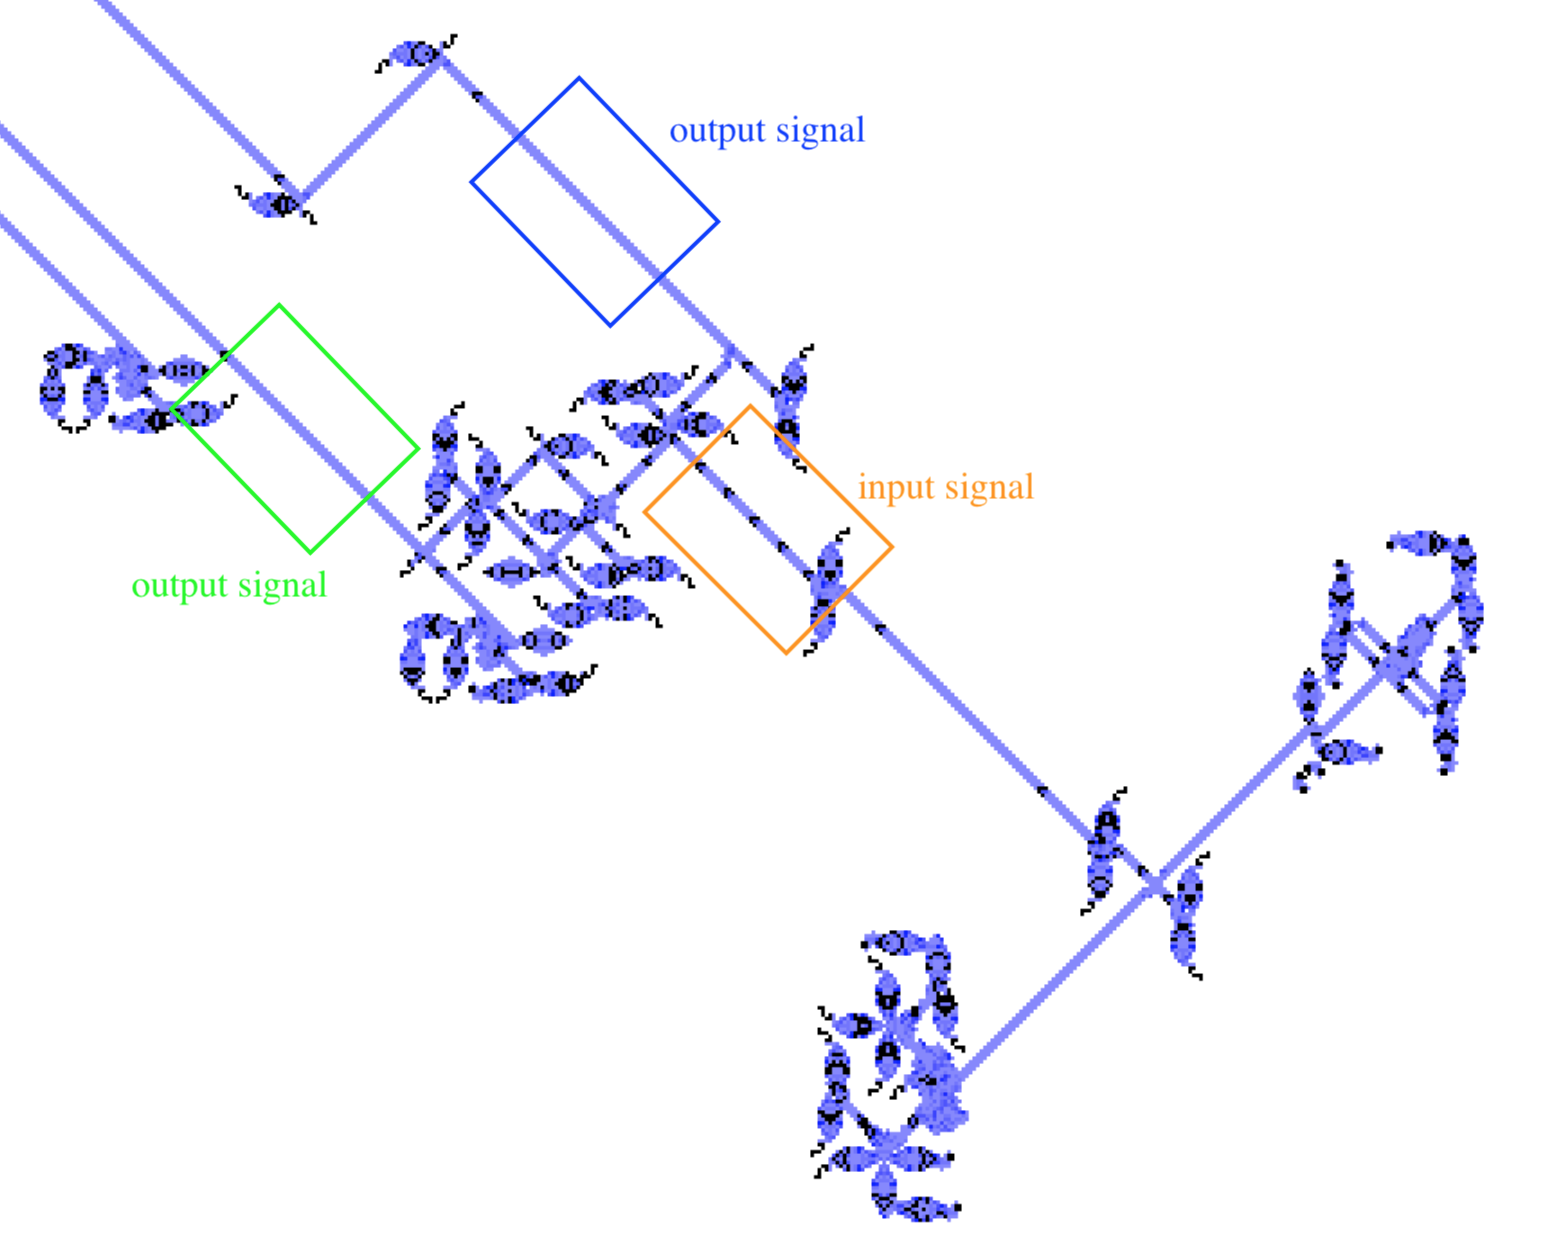
\includegraphics[width=10cm,keepaspectratio]{images/SIGNAL-DETECTOR.png}
\captionsetup{labelformat=empty} \caption{The SIGNAL DETECTOR}
\end{figure}
\subsection{Miscellaneous Components}
\noindent\textbf{1GAP$X$}: The collision of a glider with a P30 glider stream that leaves a mass that blocks altogether X gliders before disappearing. This process yields a X-glider gap in the stream. For example, a 1GAP8 is the collision of a glider with such a stream that blocks 8 gliders.

\vspace{1em}

\begin{figure}[h]
\centering
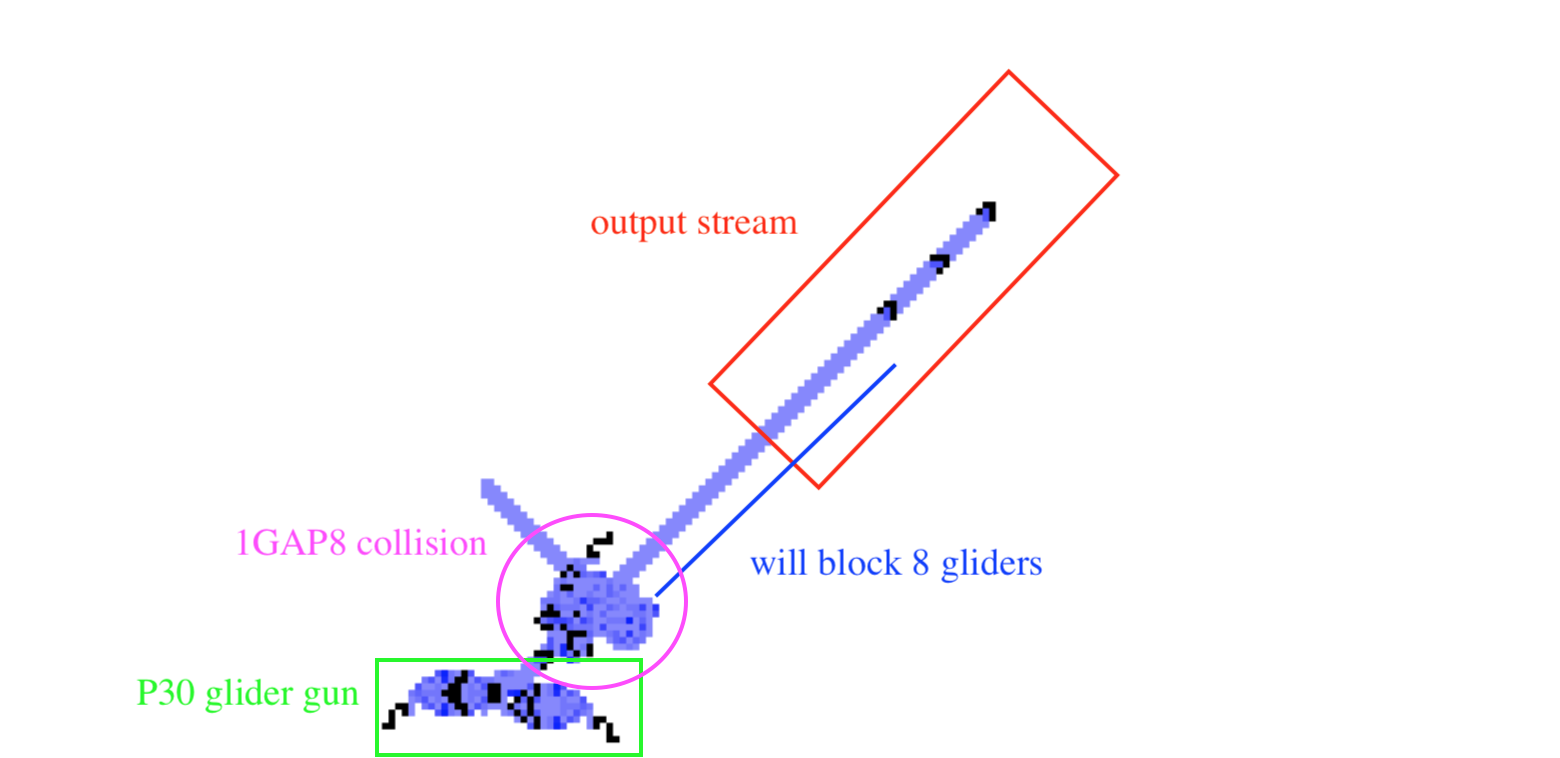
\includegraphics[width=10cm,keepaspectratio]{images/1GAP8.png}
\captionsetup{labelformat=empty} \caption{The 1GAP8 collision and effect.}
\end{figure}

\noindent\textbf{PENTADECATHLON}: An oscillator of period 15 that reflects 90-degree reflect gliders from several different angles.

\vspace{1em}

\noindent\textbf{METAMORPHOSIS II}: An oscillator of period 60 that interacts with a glider to produce a LWSS in a reflected direction from the glider.

\vspace{1em}

\noindent\textbf{FANOUT}: Receives a glider input signal from one source. After receiving a signal, FANOUT emits two glider signals perpendicular to the input signal. FANOUT has a tunable leg to adjust the input step-time.

\vspace{1em}

\begin{figure}[h]
\centering
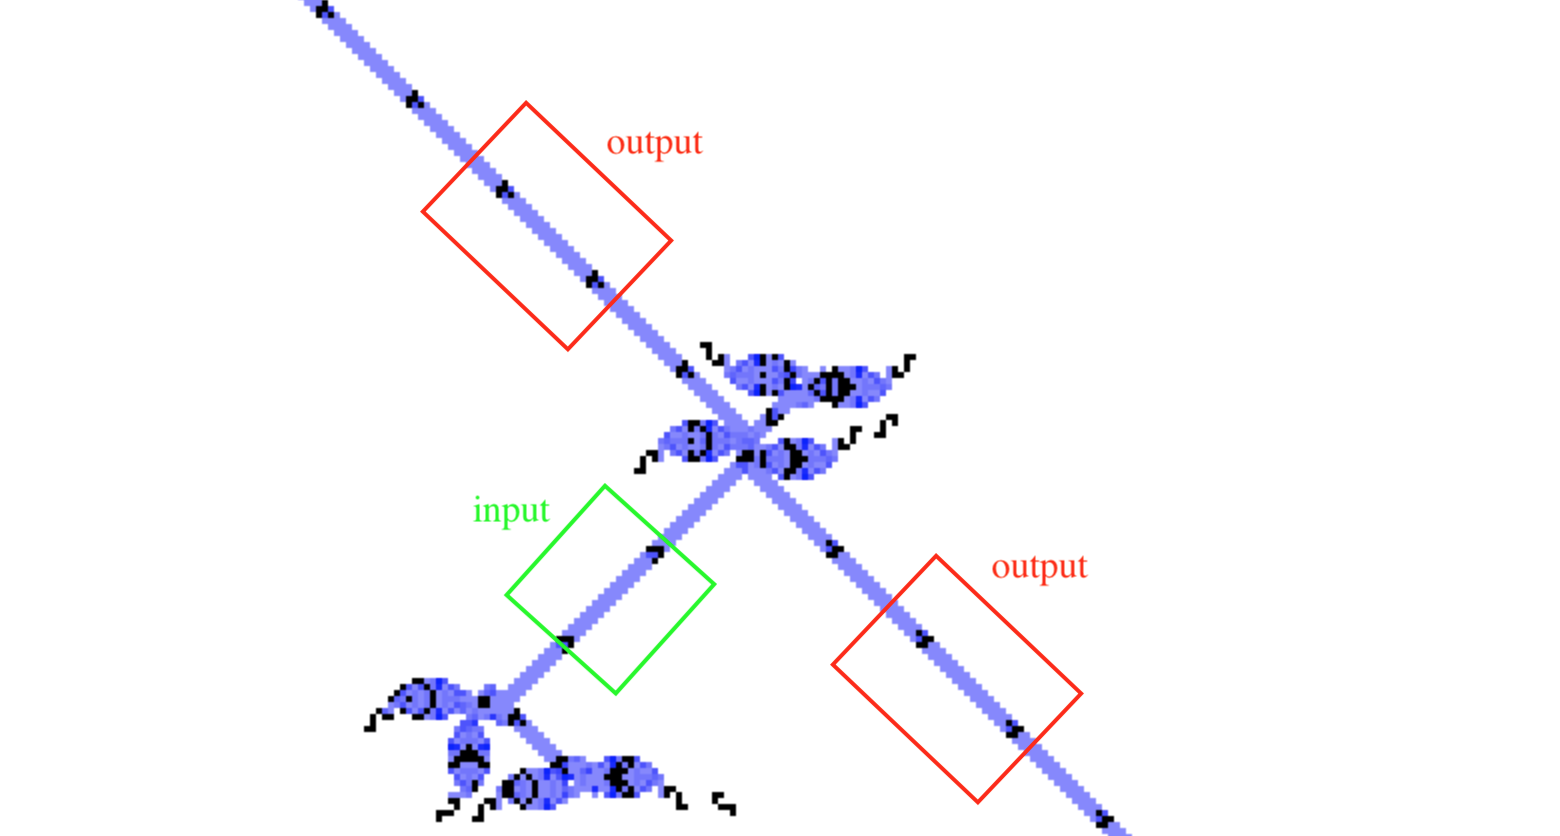
\includegraphics[width=10cm,keepaspectratio]{images/FANOUT.png}
\captionsetup{labelformat=empty} \caption{The FANOUT glider reflection pattern.}
\end{figure}
\section{Universal Computation in the Game of Life}


The Turing Machine used in the previous two sections is, notably, very simple. However, the RTM design method is capable of constructing arbitrarily-finitely-complex Turing Machines. Most importantly, a \textit{Universal Turing Machine} (UTM) is possible to construct (with the caveat, of course, that the computer simulating it has a finite amount of tape to write on).





A UTM is a Turing Machine that is capable of simulating a given Turing Machine $  M  $ on given input $  w  $. This is achieved by \textit{programming}$  M, w  $ onto the input tape for the UTM in such a way that the UTM interprets the $  M  $ and $  w  $ separately, and then simulates the running of $  M  $ on $  w  $.





The RTM specification in section 2 has a strictly-finite tape, but this turns out to be possibly transcended still within the Game of Life. The following design implements a UTM in almost entirely the same way as the original RTM, but with some arms that grow the tape as the UTM runs. As long as the tape is long enough to hold the input, the tape will grow faster than it can be written to by the UTM, and so there is effectively infinite tape-space and so it is truly a universal machine.



\begin{figure}[h]
\centering
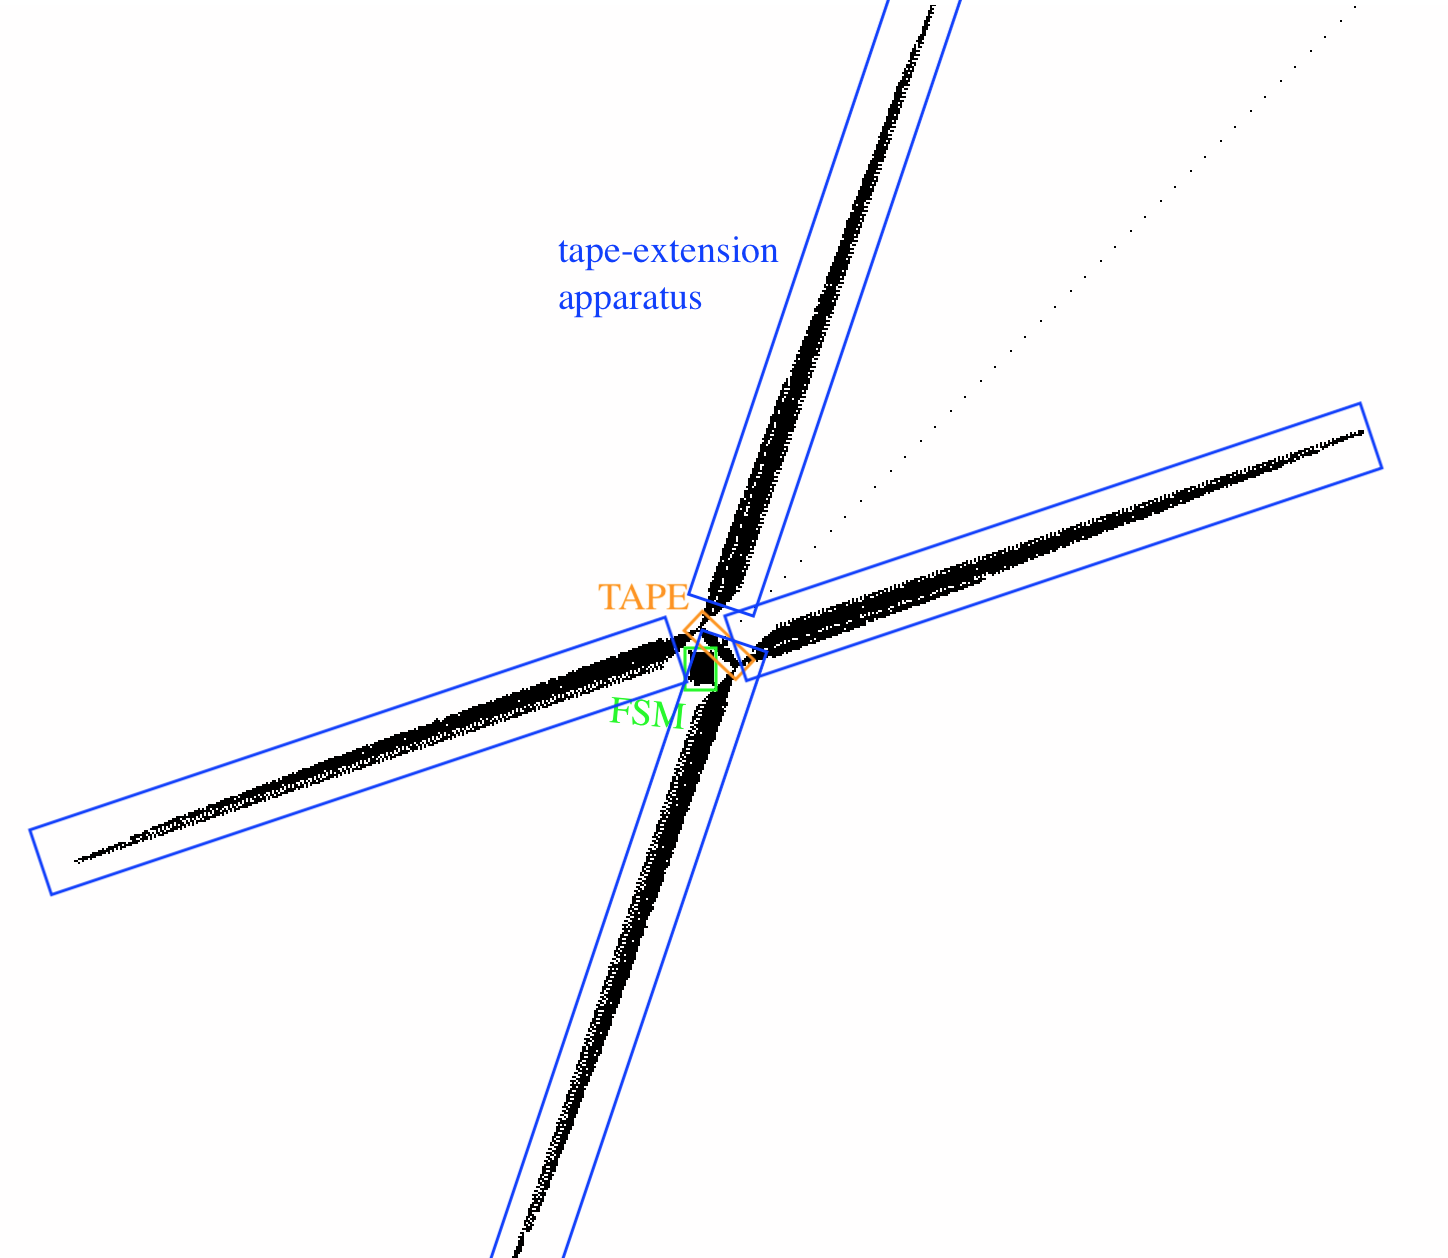
\includegraphics[width=10cm,keepaspectratio]{images/URTM-infinite.png}
\captionsetup{labelformat=empty} \caption{A UTM implemented in the Game of Life by Rendell. The spider-like arms extend the tape so that the machine has effectively infinite tape-space to compute with. The inner mechanics works the same as the RTM specification.}
\end{figure}

\begin{figure}[h]
\centering
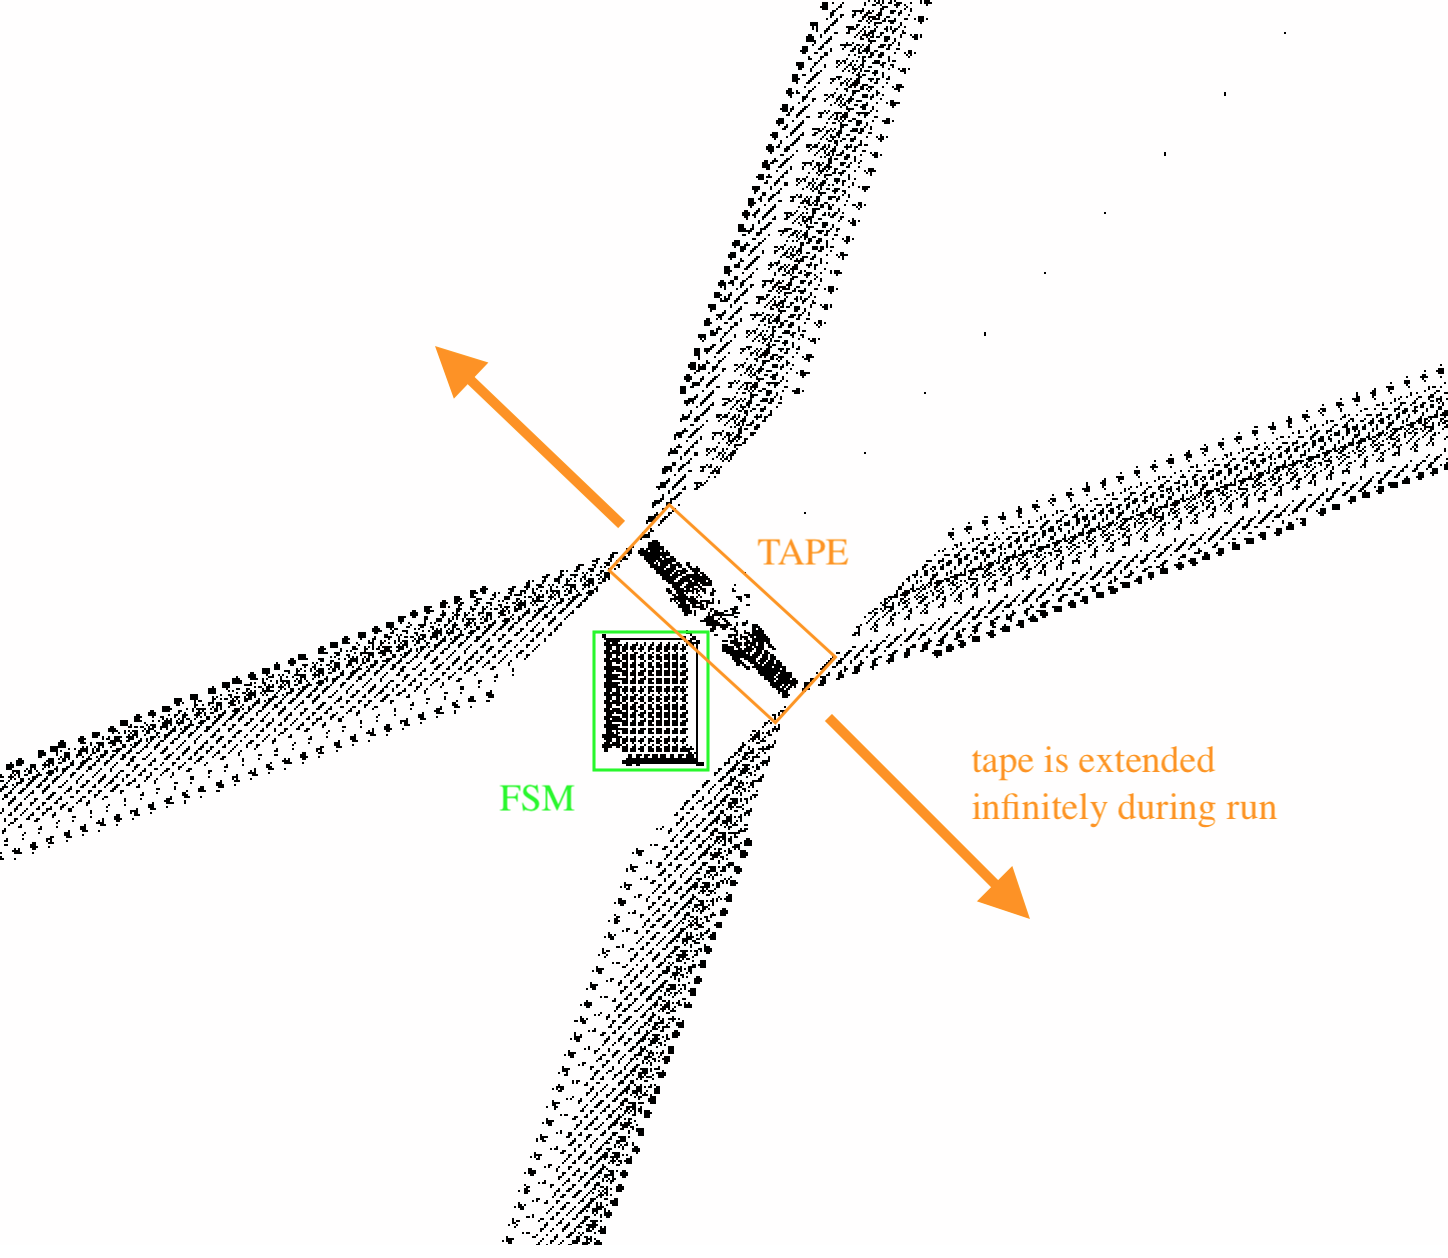
\includegraphics[width=10cm,keepaspectratio]{images/URTM-zoom.png}
\captionsetup{labelformat=empty} \caption{A close-up of the familiar mechanisms of a UTM implemented in the Game of Life by Rendell.}
\end{figure}




\section*{Bibliography}


\noindent 
  Rendell P. 2001. A Turing Machine In Conway's Game Life. [
\href{https://www.ics.uci.edu/~welling/teaching/271fall09/Turing-Machine-Life.pdf}{pdf}
]
  

\vspace*{0.2cm}


\noindent 
  Rennard J. Implementation of logical functions in the Game of Life. [
\href{http://www.rennard.org/alife/CollisionBasedRennard.pdf}{pdf}
]
  

\vspace*{0.2cm}


\noindent 
  Rendell P. 2018. Details of a Turing Machine in Conway's Game of Life. [
\href{http://rendell-attic.org/gol/tmdetails.htm}{web}
]
  

\vspace*{0.2cm}


\noindent 
  Rendell P. 2018. This is a Turing Machine implemented in Conway's Game of Life. [
\href{http://rendell-attic.org/gol/tm.htm}{web}
]
  

\vspace*{0.2cm}


\noindent 
  Rendell P. 2018. This is a Universal Turing Machine (UTM) implemented in Conway's Game of Life. [
\href{http://rendell-attic.org/gol/utm/index.htm}{web}
]
  

\vspace*{0.2cm}


\noindent 
  Rendell P. 2018. This is a Fully Universal Turing Machine (UTM) implemented in Conway's Game of Life. [
\href{http://rendell-attic.org/gol/fullutm/index.htm}{web}
]
  

\vspace*{0.2cm}


\noindent 
  LifeWiki. [
\href{http://www.conwaylife.com/wiki/}{web}
]
  

\vspace*{0.2cm}
\end{document}